\subsection{Simplicity of the alternating group ($A_n$)}
The following results are headed towards the proof of the simplicity of $A_n$ for $n \geq 5$. The 
way we will prove the simplicity of $A_n$ is by showing that every even permutation in $A_n$ can 
be expressed as a product of length-3-cycles for $n \geq 4$. Also, we will prove that every 
even permutation in $A_n$ can be expressed as a single length-3-cycle for $n \geq 5$. We will then 
say that every normal subgroup of $S_n$ that contains a length-3-cycle must contain all
length-3-cycles, hence every non-trivial normal subgroup of $A_n$ will contain at least 
one length-3-cycle, hence it will contain all of them, and so with their products, thus it 
will contain all even permutations, hence it will be equal to $A_n$. \\  

\begin{definition}[Simple group]
    A group $G$ is called simple if it has no non-trivial normal subgroups. In other words, the only 
    normal subgroups of $G$ are itself and $\{\epsilon\}$.
\end{definition} \vspace{0.2em}

\begin{theorem}
    If that $A_n$ is simple, There is no other non-trivial normal subgroup of $S_n$
\end{theorem}
\begin{proof}
    Let $H$ be a normal subgroup of $S_n$. Then, by lemma \ref{lem:intersectionOfNormalIsNormal}, we 
    have that $H \cap A_n$ is a normal subgroup of $A_n$ and since $A_n$ is simple, we have that 
    $H \cap A_n = \{\epsilon\}$ or $H \cap A_n = A_n$. \\

    If $H \cap A_n = \{\epsilon\}$, then $H$ is either the trivial subgroup or it is a group 
    with only odd permutations. Since $H$ must be a group, it must be closed under the 
    product of permutations, so it must contain the product of two odd permutations, which is an
    even permutation. Hence $H$ must contain an even permutation, which is a contradiction. \\

    If $H \cap A_n = A_n$, then $H$ contains $A_n$, so either they are identical or there 
    is an element of $S_n$ which is in $H$ but not in $A_n$. Suppose that $H$ is not
    identical to $A_n$. Then, the only element of $H$ that is not in $A_n$ must be an odd 
    permutation $\alpha$, but since $H$ is a group, it must be closed under the product of
    permutations, so it must contain $\alpha(A_n)$ which is to say that it has to contain 
    all products of even permutations with $\alpha$. \\  

    So we have that $H$ contains $\vv{f}(A_n)$ where $f$ is a function that takes an even
    permutation and returns itself multiplied by $\alpha$. The function is injective:

    $$ f(\sigma) = f(\tau) $$
    $$ \sigma \circ \alpha = \tau \circ \alpha  $$
    $$ \sigma \circ \alpha \circ \alpha^{-1} = \tau \circ \alpha \circ \alpha^{-1} $$
    $$ \sigma = \tau $$
    
    Also, since $f(\sigma)$ is an odd permutation, we can say that $\vv{f}(A_n)$ disjoint 
    from $A_n$. This means that $H$ contains two disjoint sets of permutations, both of which are
    of cardinality $|A_n|$ which implies that $|H| = 2|A_n| = |S_n|$ Hence $H$ is itself just $S_n$. \\

\end{proof} 
\vspace{0.4em}

\newpage

\begin{lemma}
    Every even permutation in $A_n$ of length 2 can be expressed 
    as a product of length-3-cycles for $n \geq 4$.
\end{lemma}
\begin{proof}
    We can express every even permutation of length 2 in the form $(a,b) \circ (b,c)$ 
    as the product of two length-3-cycles $(a,b,c) \circ (1)$. So, without loss of generality,
    we can focus just on permutations of the form $(a,b) \circ (c,d)$.\\

    We can easily show that every permutation in the form $(a,b) \circ (b,c)$ can be 
    expressed as the product of multiple legth-3-cycles as shown below in figres \ref{fig:SwapTwo} and 
    \ref{fig:SwapTwoAs3Cycles} \\
\end{proof} \vspace{0.2em}

\begin{figure}[H]
\label{fig:SwapTwo}
    \centering
    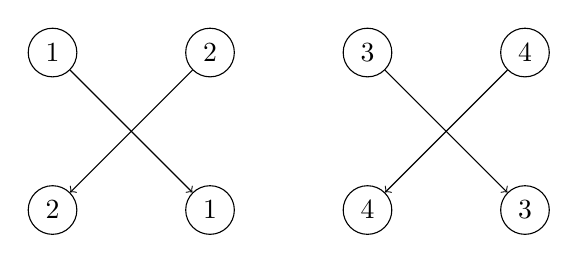
\begin{tikzpicture}
        
        \node (1-1) at (0, 0) [circle, draw] {1};
        \node (1-2) at (2, 0) [circle, draw] {2};
        \node (1-3) at (4, 0) [circle, draw] {3};
        \node (1-4) at (6, 0) [circle, draw] {4};
        
        \node (2-1) at (0, -2) [circle, draw] {2};
        \node (2-2) at (2, -2) [circle, draw] {1};
        \node (2-3) at (4, -2) [circle, draw] {4};
        \node (2-4) at (6, -2) [circle, draw] {3};

        \draw[->] (1-1) -- (2-2);
        \draw[->] (1-2) -- (2-1); 

        \draw[->] (1-3) -- (2-4);
        \draw[->] (1-4) -- (2-3); 

    \end{tikzpicture}
    \caption{The permutation $[(1,2) \circ (3,4)]$ }

\end{figure}

\begin{figure}[H]
\label{fig:SwapTwoAs3Cycles}
    \centering
    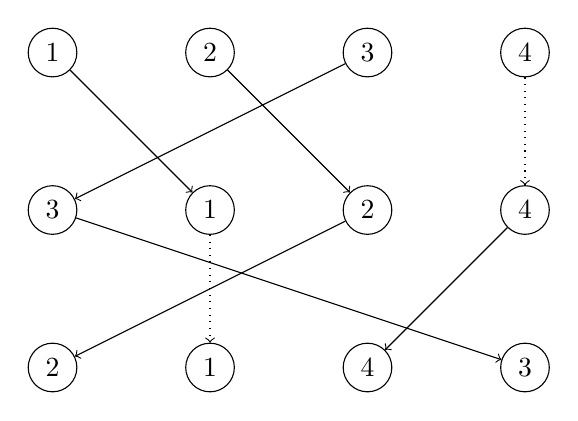
\begin{tikzpicture}
        
        \node (1-1) at (0, 0) [circle, draw] {1};
        \node (1-2) at (2, 0) [circle, draw] {2};
        \node (1-3) at (4, 0) [circle, draw] {3};
        \node (1-4) at (6, 0) [circle, draw] {4};
        
        \node (2-1) at (0, -2) [circle, draw] {3};
        \node (2-2) at (2, -2) [circle, draw] {1};
        \node (2-3) at (4, -2) [circle, draw] {2};
        \node (2-4) at (6, -2) [circle, draw] {4};

        \node (3-1) at (0, -4) [circle, draw] {2};
        \node (3-2) at (2, -4) [circle, draw] {1};
        \node (3-3) at (4, -4) [circle, draw] {4};
        \node (3-4) at (6, -4) [circle, draw] {3};

        \draw[->] (1-1) -- (2-2);
        \draw[->] (1-2) -- (2-3);
        \draw[->] (1-3) -- (2-1);
        \draw[dotted, ->] (1-4) -- (2-4);
        
        \draw[->] (2-1) -- (3-4);
        \draw[dotted, ->] (2-2) -- (3-2);
        \draw[->] (2-4) -- (3-3);
        \draw[->] (2-3) -- (3-1); 
 

    \end{tikzpicture}
    \caption{The permutation $[(1,2,3) \circ (1,4,3)]$ }

\end{figure} \vspace{0.4em}

\begin{lemma}
    \label{lem:evenPermutationIsProductOfThreeCycles}
    Every even permutation in $A_n$ of arbitraty length can be expressed 
    as a product of length-3-cycles for $n \geq 4$.
\end{lemma}
\begin{proof}
    By definition, every even permutation of length $2k$ is a product of $2k$ length-2-cycles, which 
    are called prime-factors. We can consider them pairwise and define every even permutation 
    as a product of $k$ even permutations of length 2. Thanks to lemma 
    \ref{lem:evenPermutationIsProductOfThreeCycles} we can herby
    express every even permutation of length $2k$ as a product of $k$ length-3-cycles,
    thus proving the lemma. \\
\end{proof} \vspace{0.2em}

\newpage

\begin{lemma}
    \label{lem:everyThreeCycleIsInSubgroupsOfAN}
    Every normal subgroup $H \triangleleft S_n$ that contains a length-3-cycle must contain all 
    length-3-cycles given that $n \geq 3$.
\end{lemma}
\begin{proof}
    Assume $H \triangleleft S_n$ and that $H$ contains a length-3-cycle $(a,b,c)$. Then consider 
    that by definition of normality we have that the following statement holds true:

    $$ \forall \pi \in S_n\;\; \pi \circ (a,b,c) \circ \pi^{-1} \in H $$ \vspace{0.2em}

    We want to show that $H$ contains all length-3-cycles. So, for the arbitrary length-3-cycle
    $(i,j,k)$ we will show that we can find a permutation $\pi$ such that:

    $$ \pi \circ (a,b,c) \circ \pi^{-1} = (i,j,k) $$ \vspace{0.2em}

    In particular, such permutation $\pi$ exists and its defined by cases as shown below:

    \begin{equation*}
        \pi(x) = 
        \begin{cases*}
            a      & \text{if} \( x = i \)  \\
            b      & \text{if} \( x = j \)  \\
            c      & \text{if} \( x = k \)  \\
            x      & \text{otherwise}       \\
        \end{cases*}
    \end{equation*} \\
\end{proof}

\begin{lemma}
    If $\pi = (a,b,c)$ is a length-3-cycle, then $\sigma \circ \pi \circ \sigma^{-1} = (i,j,k)$
    is also a length-3-cycle for every permutation $\sigma$ in $S_n$. 
\end{lemma}
\begin{proof}
   The effect of the permutation $\sigma$ is reversed by the inverse $\sigma^{-1}$, except for 
   the three elements $a$, $b$ and $c$ which are permuted by $\pi$. So $\sigma \circ \pi \circ 
   \sigma^{-1}$ is a length-3-cycle. \\


   \begin{equation*}
        \sigma \circ \pi \circ \sigma^{-1} = 
        \begin{cases*}
            \sigma^{-1}(\pi(\sigma(x)))   & \text{if} \( x \in \{a,b,c\} \)  \\
            \sigma^{-1}(\sigma(x))        & \text{otherwise}       \\
        \end{cases*}
    \end{equation*} \\

    This deconstruction makes it clear that only three elements are permuted, thus, the
    permutations of this form are all length-3-cycles. \\ 
\end{proof} \vspace{0.2em}

We will state as a fact without proof that $A_5 and A_6$ are simple groups. In canonical group theory 
courses such result gets formally proven, but we will not go into the details of such proof. Please 
keep in mind that the proof of the simplicity of $A_5$ and $A_6$ is not necessary since 
they are finite groups and it can be shown by brute-force that they have no non-trivial normal
subgroups. Modern super-computers can easily compute every subgroup of $A_6$ and check it 
effortlessly. Thus a formal proof not really necessary. \\

\newpage

To formally prove the simplicity of $A_n$, one could use either the Sylow's theorems, or 
the Lagrange's theorem, or one could go case by case and observe that every even permutation 
can being in a normal subgroup of $A_n$ implies that some other length-3-cycle must also be in
such normal subgroup. The latter is expecially tedious. \\


\begin{theorem}[Simplicity of $A_n$]
    $A_n$ is simple for $n \geq 5$.
\end{theorem}
\begin{proof}
    Proceed by induction. Since the statement is true for $n = 5$ and $n = 6$ assume it's true for 
    any n. Let $\pi = (a,b,c) \in A_3$, and let $N \triangleleft A_{n+1}$, then take 
    $\sigma \in N$.\\

    Since $\pi$ is a length-3-cycle, we can say that $\sigma \circ \pi \circ \sigma^{-1} = (i,j,k)$
    is also a length-3-cycle. By lemma \ref{lem:everyThreeCycleIsInSubgroupsOfAN}. So consider the 
    following construction:\\

    $$ (\sigma^{-1} \circ \pi \circ \sigma) \circ \pi^{-1} = (i,j,k)(a,b,c) $$
    $$ \sigma^{-1} \circ (\pi \circ \sigma \circ \pi^{-1}) \in N $$ \\

    By definition of normality, since $\sigma \in N$, the permutation $(\pi \circ \sigma \circ \pi^{-1})$ 
    must also be in $N$. So the product of $\sigma^{-1}$ with such permutation is also still in $N$. \\

    Notice that the product of two length-3-cycles is in $A_6$ since it's even by definition and 
    it permutes at most 6 elements. So we can say that $N \subseteq A_6$. Since $A_6$ is simple,
    the intersection $A_6 \cap N$ is either trivial or $A_6$. Since $N$ contains an even permutation
    that is in $A_6$ it must be a superset of $A_6$. So it must contain some length-3-cycles. \\

    Via lemma \ref{lem:everyThreeCycleIsInSubgroupsOfAN} we can say that $N$ contains all
    length-3-cycles, hence by lemma \ref{lem:evenPermutationIsProductOfThreeCycles} we can say 
    that $N$ contains all even permutations. Hence $N = A_{n+1}$. \\
\end{proof} \vspace{0.2em}
    
This proof in particular is attributed to the mathematician \textbf{Joseph Gallian}, and it's a much 
more concise proof than the one given by \textbf{Galois} in his original paper. It is possible 
to improve this proof by reducing the necessary assumptions to the fact that $A_5$ is simple, thus 
ignoring the case of $A_6$. \\

In the next chapter we will talk about Galois-solvability of a given group, and how the fact that 
$A_n$ is non-abelian and simple for $n \geq 5$ implies that the group $S_n$ is not 
Galois-solvable for $n \geq 5$. This will later be used to prove that there is no such thing 
as the quintic formula. \\

\newpage
